% !TEX TS-program = pdflatex
% !TEX encoding = UTF-8 Unicode

% This is a simple template for a LaTeX document using the "article" class.
% See "book", "report", "letter" for other types of document.

\documentclass[12pt,a4paper,titlepage]{scrartcl} % use larger type; default would be 10pt

\usepackage[utf8x]{inputenc} % set input encoding (not needed with XeLaTeX)

%%% Examples of Article customizations
% These packages are optional, depending whether you want the features they provide.
% See the LaTeX Companion or other references for full information.

%%% PAGE DIMENSIONS
\usepackage{geometry} % to change the page dimensions
%\geometry{a4paper} % or letterpaper (US) or a5paper or....
\geometry{bottom=3.5cm} % for example, change the margins to 2 inches all round
% \geometry{landscape} % set up the page for landscape
%   read geometry.pdf for detailed page layout information

\usepackage{graphicx} % support the \begin{center}\includegraphics command and options
\usepackage{wrapfig}

% \usepackage[parfill]{parskip} % Activate to begin paragraphs with an empty line rather than an indent

%%% PACKAGES
%\usepackage{booktabs} % for much better looking tables
%\usepackage{array} % for better arrays (eg matrices) in maths
\usepackage{paralist} % very flexible & customisable lists (eg. enumerate/itemize, etc.)
%\usepackage{verbatim} % adds environment for commenting out blocks of text & for better verbatim
%\usepackage{subfig} % make it possible to include more than one captioned figure/table in a single float
% These packages are all incorporated in the memoir class to one degree or another...
\usepackage[ngerman]{babel}
\usepackage{pifont} %for symbols (i.e. arrows)
\usepackage{fancyhdr}
%\usepackage{showframe} %shows the margins

\usepackage[colorlinks]{hyperref} % package for hyperlinks with \url
\usepackage[svgnames]{xcolor}
\usepackage[anythingbreaks]{breakurl}

%%redifine of emph, see http://tex.stackexchange.com/questions/6754/what-is-the-canonical-way-to-redefine-the-emph-command
\makeatletter
\DeclareRobustCommand{\em}{%
  \@nomath\em \if b\expandafter\@car\f@series\@nil
  \normalfont \else \bfseries \fi}
\makeatother

%%% HEADERS & FOOTERS
%set with fancy layout package
\usepackage{fancyhdr} % This should be set AFTER setting up the page geometry
\pagestyle{fancy} % options: empty , plain , fancy
\renewcommand{\headrulewidth}{0pt} % customise the layout...
\lhead{}\chead{}\rhead{}
\lfoot{}\cfoot{\thepage}\rfoot{}

\setlength{\parindent}{0mm} %set paragraph begin indentation to 0

% hyperlink color definitions
\hypersetup{citecolor=DeepPink4}
\hypersetup{linkcolor=DarkRed}
\hypersetup{urlcolor=DarkBlue} 

%%% SECTION TITLE APPEARANCE
\usepackage{sectsty}
\allsectionsfont{\sffamily\mdseries\upshape} % (See the fntguide.pdf for font help)
% (This matches ConTeXt defaults)

%%% ToC (table of contents) APPEARANCE
%\usepackage[nottoc,notlof,notlot]{tocbibind} % Put the bibliography in the ToC
%\usepackage[titles,subfigure]{tocloft} % Alter the style of the Table of Contents
%\renewcommand{\cftsecfont}{\rmfamily\mdseries\upshape}
%\renewcommand{\cftsecpagefont}{\rmfamily\mdseries\upshape} % No bold!

%%% END Article customizations

%%% The "real" document content comes below...

\title{Videostreaming mit dem Raspberry Pi und der Raspberry Pi Camera}
\author{Sebastian Deußer}
%\date{2. April 2014} % Activate to display a given date or no date (if empty),
         % otherwise the current date is printed 
\setcounter{section}{-1}

\begin{document}
\maketitle %title (page)

%header and footer definitions for fancyhdr
\pagestyle{fancy}
\lhead{}
\chead{\leftmark}
\rhead{}
\lfoot{Sebastian Deußer}
\cfoot{}
\rfoot{Seite \thepage}

\thispagestyle{fancy}

\section{Vorbereitungen}
Wir haben auf unserem Raspberry Pi das Raspbian System laufen. In raspi-config haben wir die Kamera angeschaltet. Für Methode 2 muss man zusätzlich zu den Standard-Paketen noch vlc installieren.
	\begin{center}
		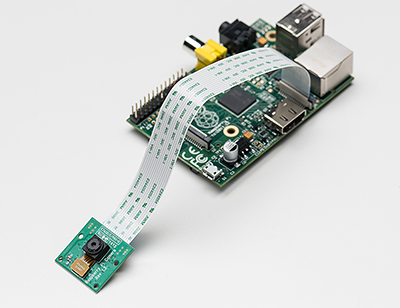
\includegraphics[height=9cm]{Streaming/1367_MED}
	\end{center}
Die Raspberry Pi Kamera muss wie auf dem Foto zu sehen ist angeschlossen werden, mit den Kontakten des Flachbandkabels Richtung HDMI-Port. Beim Einbau muss man etwas vorsichtig sein da die Kamera empfindlich ist gegen elektrostatische Entladungen.

\newpage
\section{Methode 1: Mit MJPG-Streamer}
\small{(Quelle: \href{http://blog.miguelgrinberg.com/post/how-to-build-and-run-mjpg-streamer-on-the-raspberry-pi}{http://blog.miguelgrinberg.com/post/how-to-build-and-run-mjpg-streamer-on-the-raspberry-pi})}
\normalsize

\begin{enumerate}
\bfseries

\item build Abhängigkeiten von mjpg-streamer installieren:\newline
\texttt{\$ sudo apt-get install libjpeg8-dev imagemagick libv4l-dev}

\item Symlink für fehlende videodev.h setzen:\newline
\textnormal{Die videodev.h Header Datei die MJPG-Streamer benötigt wurde durch \mbox{videodev2.h} ersetzt. Um MJPG-Streamer trotzdem glücklich zu machen muss man folgenden symbolischen Link erstellen:}\newline
\texttt{\$ sudo ln -s /usr/include/linux/videodev2.h /usr/include/linux/videodev.h}

\item Download MJPG-Streamer:\newline
\textnormal{Der Quellcode für MJPG-Streamer ist bei sourceforge.net erhältlich, aber ein direkter Download-Link ist etwas schwierig zu bekommen:}\newline
\texttt{\$ wget \url{http://sourceforge.net/code-snapshots/svn/m/mj/mjpg-streamer/code/mjpg-streamer-code-182.zip}}

\item MJPG-Streamer Quellcode entpacken:\newline
\textnormal{Der downgeloadete Quellcode ist ein gepacktes zip file. Entpacke die Datei im Home-Verzeichnis (oder in einem temporären Verzeichnis):}\newline
\texttt{\$ unzip mjpg-streamer-code-182.zip}

\item MJPG-Streamer bauen:\newline
\textnormal{MJPG-Streamer hat einige Plugins, aber nur ein paar davon werden hier benötigt. Folgender Befehl baut nur das Nötigste:}\newline
\texttt{\$ cd mjpg-streamer-code-182/mjpg-streamer\newline
\$ make mjpg\_streamer input\_file.so output\_http.so}

\item MJPG-Streamer installieren:\newline
\textnormal{Die folgenden Befehle installieren das gebaute Programm:}\newline
\texttt{\$ sudo cp mjpg\_streamer /usr/local/bin\newline
\$ sudo cp output\_http.so input\_file.so /usr/local/lib/\newline
\$ sudo cp -R www /usr/local/www}

\item Starte die camera:\newline
\textnormal{Nun ist es Zeit das Kamera-Modul anzuwerfen:}\newline
\texttt{\$ mkdir /tmp/stream\newline
\$ raspistill --nopreview -w 640 -h 480 -q 5 -o /tmp/stream/pic.jpg -tl 100 -t 9999999 -th 0:0:0 \&}\newline
\textnormal{Natürlich kann man raspistill auch mit anderen Optionen starten.}

\item Starte MJPG-Streamer:\newline
\textnormal{Die Kamera schreibt nun Bilder, man muss nur noch MJPG-Streamer starten:}\newline
\texttt{\$ LD\_LIBRARY\_PATH=/usr/local/lib mjpg\_streamer -i \char`\"input\_file.so -f /tmp/stream -n pic.jpg\char`\" -o \char`\"output\_http.so -w /usr/local/www\char`\"} % \char`\" is a crude hack for straight quotation marks

\item Schau den Stream an!\newline
\textnormal{Nun kann man sich über einen Web-Browser verbinden und den Live-Stream ansehen. Man kann ihn vom Raspberry Pi selbst per Eingabe von \url{http://localhost:8080} in der Browser-Adresszeile ansehen. Oder wenn man ihn von einem anderen Rechner im Netzwerk ansehen will muss man \url{http://<IP-Adresse>:8080} aufrufen.}\newline
	    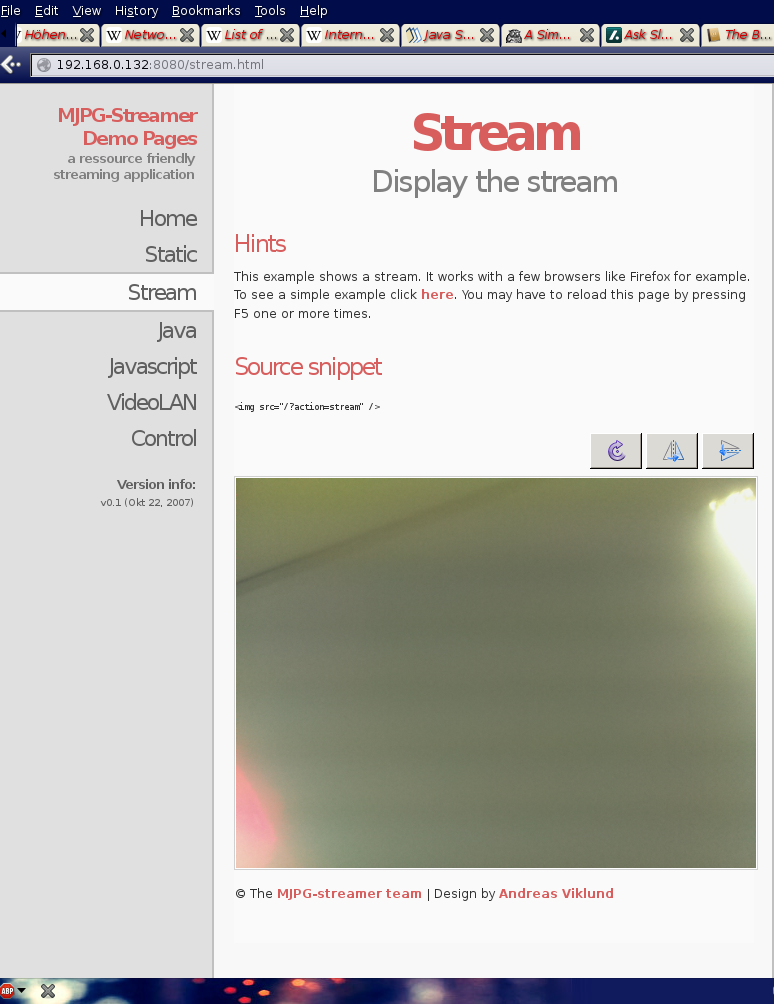
\includegraphics[width=0.6\textwidth]{Streaming/MJPG-Streamer_cut}

\item Aufräumen:\newline
\textnormal{Nachdem man überprüft hat das alles geht kann man den Quellcode wieder löschen, er wird nicht mehr benötigt.}\newline
\texttt{\$ cd ../../\newline
\$ rm -rf mjpg-streamer-182}
\end{enumerate}
\end{document}
